\section{Introduction}
\label{AABB_tree_section_intro}

The AABB tree component offers a static data structure and algorithms to perform efficient intersection and distance queries against sets of 3D geometric objects.
The set of geometric objects stored in the data structure may be queried for intersection detection, intersection computation and distance queries with any type of query, provided that the corresponding intersection and distance predicates and constructors are implemented in the traits class.\\

Examples of intersection queries include line objects (rays, lines or segments) against sets of triangles, or plane objects (planes or triangles) against sets of segments. An example of distance query consists of finding the closest point from a point query to a set of triangles.\\

The AABB tree data structure takes as input an iterator range of geometric data, which are then converted into primitives, where each primitive gives access to both one input geometric object (so-called datum) and one reference id to this object (e.g., wraps a 3D triangle and a face handle of a polyhedral surface). The reference id is used by the AABB tree to refer to the primitive in the results provided to the user. Note that these reference ids need not be unique: several primitives may share the same id. From these primitives a hierarchy of axis-aligned bounding boxes (AABBs) is constructed and used to speed up intersection and distance queries (see Figure~\ref{fig:AABB-tree-anchor}). 

\begin{center}
    \label{fig:AABB-tree-anchor}
    \begin{ccTexOnly}
      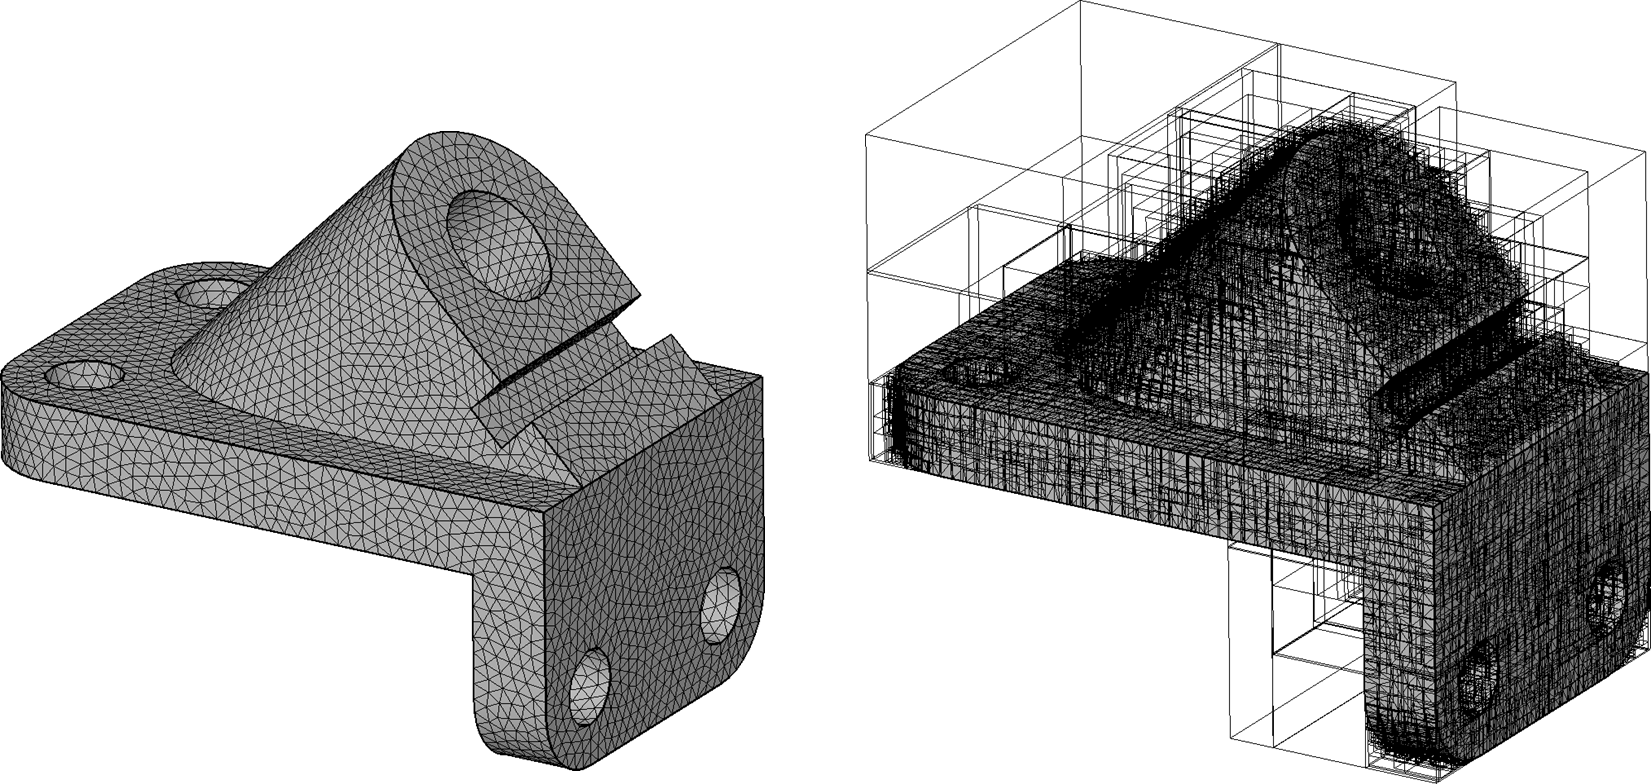
\includegraphics[width=1.0\textwidth]{AABB_tree/anchor}
    \end{ccTexOnly}
    \begin{ccHtmlOnly}
        <img width="99%" border=0 src="./anchor.png"><P>
    \end{ccHtmlOnly}
    \begin{figure}[h]
        \caption{AABB tree.
                 Left: surface triangle mesh of a mechanical part.
                 Right: AABB tree constructed.}
    \end{figure}
\end{center}
